\chapter{Implementation}
Write in detail about how i solved the task

\section{RFID circuit design}
The full circuit for one RFID node can be found in \ref{appendix:RFIDreader}. An approach where one PCB for each row was chosen, for ease of installation.
\subsection{Resonance circuit}

In order to power a passive tag, we need some form of resonance circuit that will resonate with the passive tag. We are choosing the 125 kHz frequency, hence the circuit needs to resonate at this frequency. The coils that were available was measured to 500$\mu$H $\pm$ 20 $\mu$H as shown in figure \ref{fig:05:henry}. The resonance frequency of an LC circuit can be found from the following formula:
\begin{align}
    2*\pi*F=\frac{1}{\sqrt{L*C}}
\end{align}
Where F is frequency, L is inductance in Henry and C is capacitance in Farad. Both the Frequency we need and the value of the coil is fixed, so the only variable is the capacitor. Rearranging the formula we get:

\begin{align}
    C&=\Big(\frac{1}{2\pi*F}\Big)^2-L\\
    C&\approx 3.24nF
\end{align}

3.24nF is not a standard value for a capacitor, and very accurate capacitors are expensive. The closest standard value is 3.3nF. Fortunately we are only in the kilohertz spectre, meaning a slightly "off" capacitor will not cause major problems. The capacitors used are $\pm$ 10\% which will give a worst case of 2.97nF and 3.63nF which correspond to resonance at 131 kHz and 118 kHz. This will only result in a weaker resonance, as the generator will run at 125kHz regardless of the actual capacitor value, resulting only in a shorter read distance.



\begin{figure}[h]
    \centering
    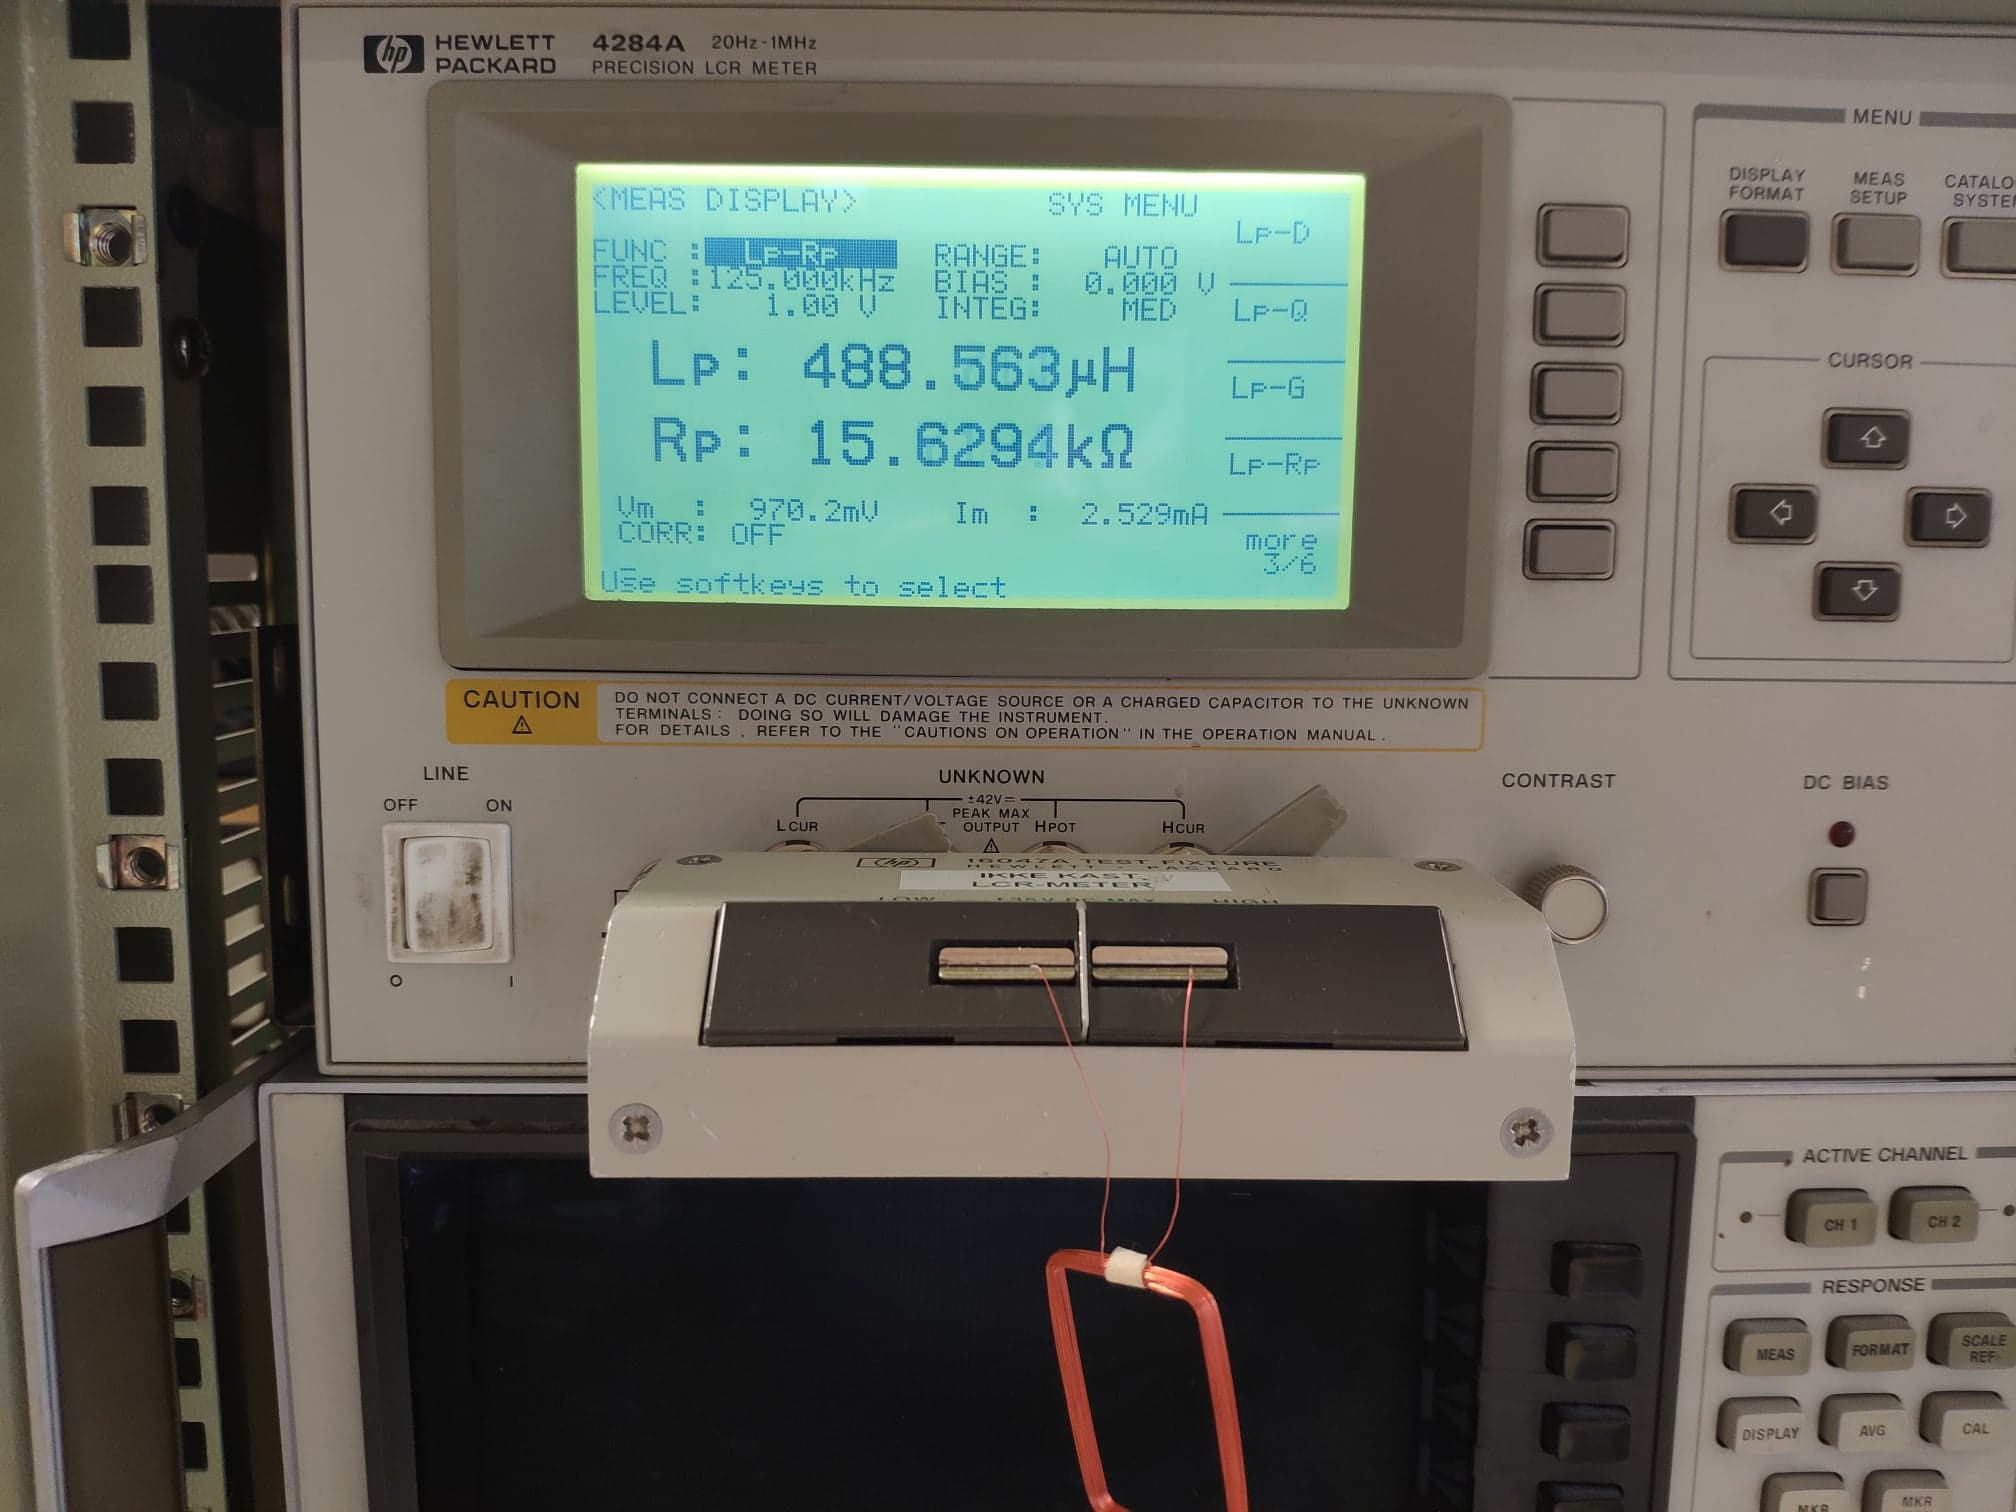
\includegraphics[width=\textwidth]{05_My_Implementation/figures/Coil_henry.jpg}
    \caption{LCR readout of one of the coils at 125 kHz}
    \label{fig:05:henry}
\end{figure}

\begin{figure}[h]
    \centering
    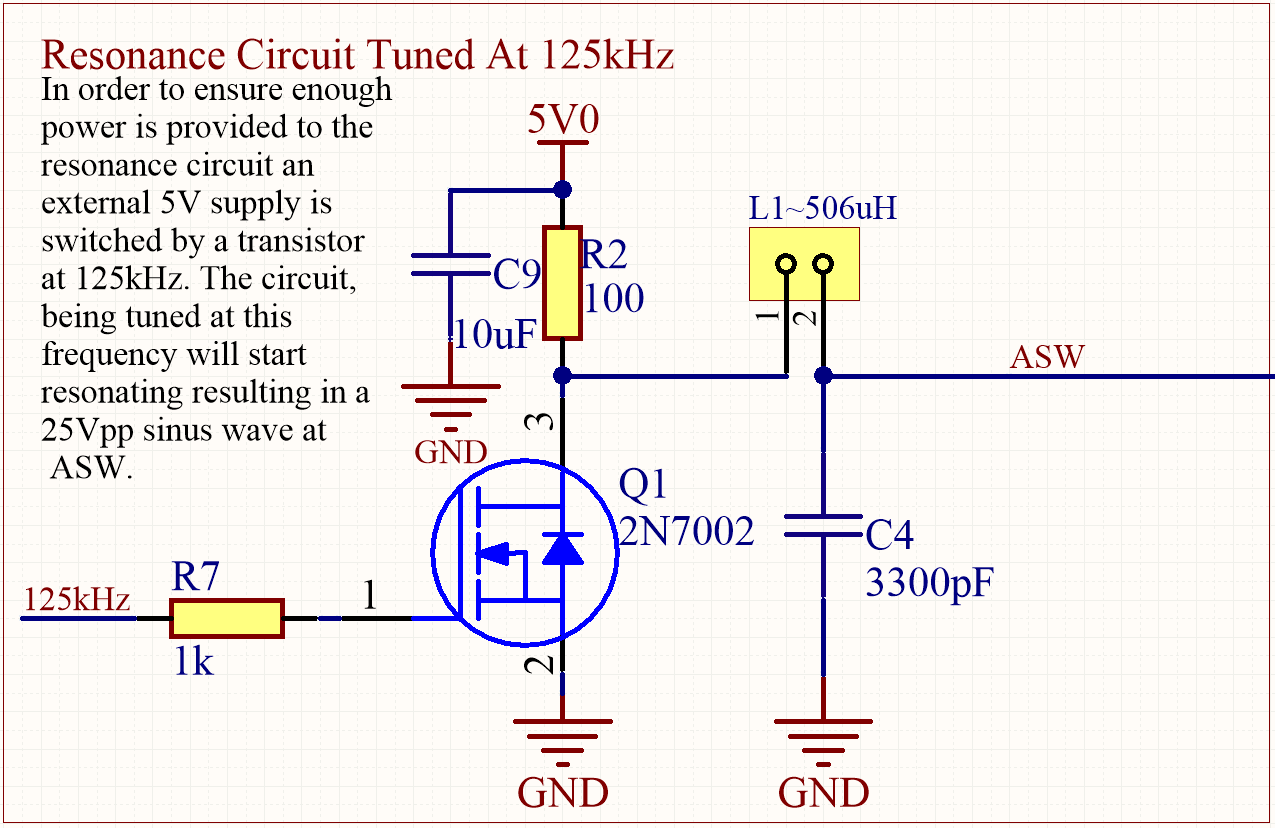
\includegraphics[width=\textwidth]{05_My_Implementation/figures/Resonance_circuit.png}
    \caption{Resonance circuit schematic snippet}
    \label{fig:05:Resonance_circuit}
\end{figure}

As seen in figure \ref{fig:05:Resonance_circuit} R7 is to protect the MCU from ESD from the resonance circuit. Q1 will pull the resonance circuit to ground when open and effectively drive it at 125kHz. R2 is helping limiting the current drawn by the circuit. L1 and C4 are the coil and capacitor respectively.

\newpage\newpage
\subsection{Peak detector}
When the passive RFID tag is present in the magnetic field produced by the resonance circuit, it will leech a little power from it in a distinct pattern. It is only these changes in voltage that is useful to us. By saturating the capacitor C2, and subsequently let it bleed out over R5  quickly enough to drop to "active load" for the tag we get a square wave from of the tags ID. The diode D1 is there to to ensure no negative voltage further into the system and keeping the integrity of the signal.

\begin{figure}[h]
    \centering
    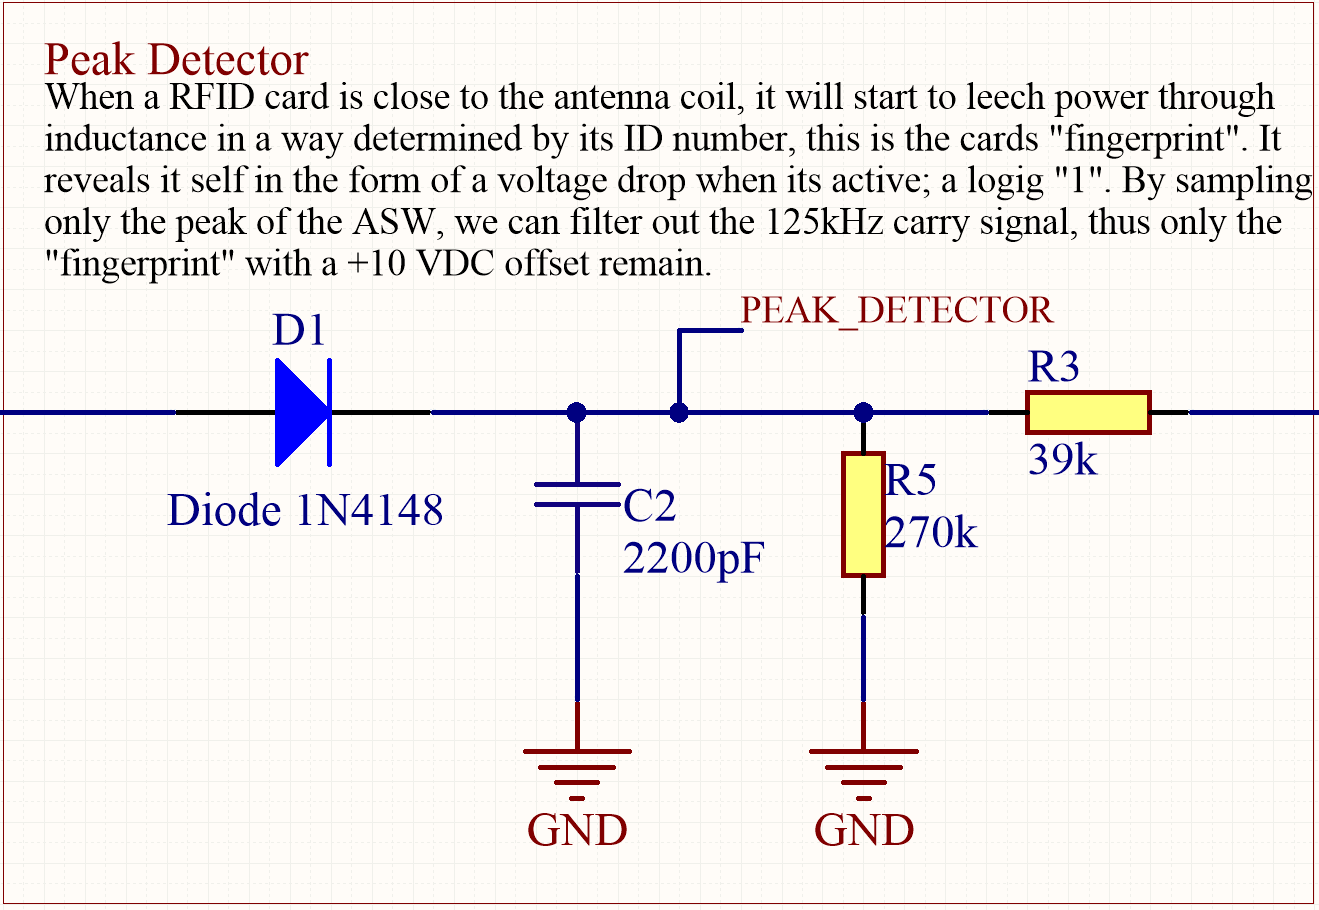
\includegraphics[width=\textwidth]{05_My_Implementation/figures/Peak_detector.png}
    \caption{Schematic of a simple peak detector}
    \label{fig:05:peak}
\end{figure}
\clearpage
\subsection{DC-block}
Due to the resonance we get approximately 25Vpp on the carry wave, given the diode we will only have the positive part, so around 12,5V in the peak detector. In order to cut out this DC offset a DC-block is introduced, only letting the AC component through. Depending on how good the tag resonates with the reader, the Vpp of this AC component can be everything form a meager 800 mV to 4 V. The tags used in the implementation of this system typically came out around 1.5 V peak-to-peak as can be seen in the results section. 
\begin{figure}[H]
    \centering
    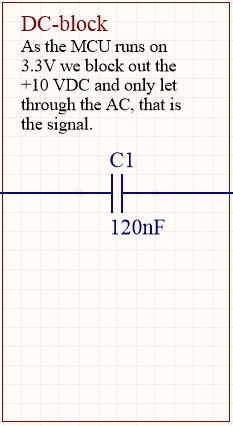
\includegraphics[width=0.3\textwidth]{05_My_Implementation/figures/DC_block.png}
    \caption{DC-Block}
    \label{fig:my_label}
\end{figure}
\clearpage
\subsection{Voltage divider}
Given the difference in resonance in tags, a fixed small DC offset can be useful, this way, we know that the signal will oscillate around this offset, making the reading process more predictable. 
\begin{figure}[h]
    \centering
    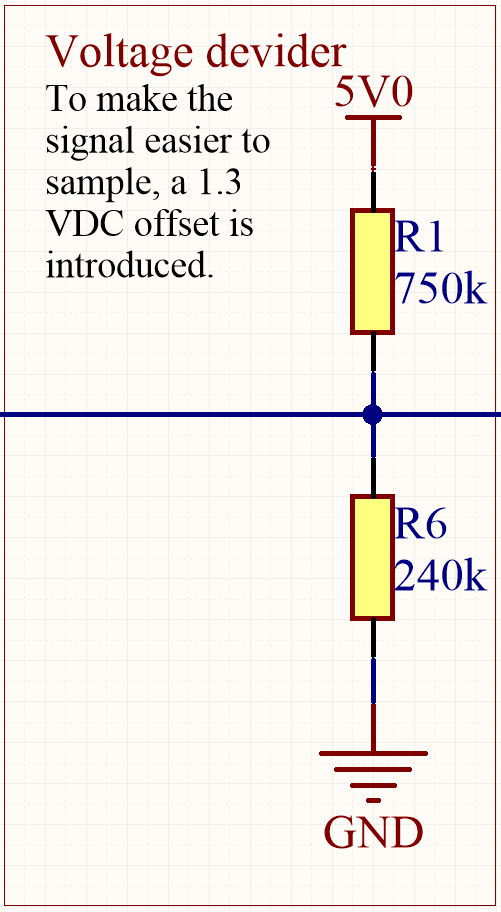
\includegraphics[width=0.3\textwidth]{05_My_Implementation/figures/Voltage_division.png}
    \caption{Voltage divider ensuring a known DC offset}
    \label{fig:my_label}
\end{figure}

\subsection{Low pass filter}
The 125 kHz carry signal , even though modulated by the tag, will be present still in the modulated signal. this in the form of a ripple on the modulated signal, noise. The maximum hysteresis on the AC of the ATtiny1617 is 50mV. A low pass filter will mitigate the bulk of this ripple, but we will trade this in for a slower rise and fall time. This can be seen in the results. 
\begin{figure}[H]
    \centering
    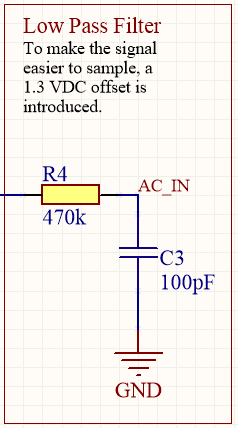
\includegraphics[width=0.3\textwidth]{05_My_Implementation/figures/LPF.png}
    \caption{Low pass filter, smoothing out the signal before going in to the AC}
    \label{fig:my_label}
\end{figure}

\subsection{TWI and SPI}
Two Wire Interface, Microchips I$^2$C compatible module is implemented in a way which allows for physical setting of its ID, this way we only need to write the code once, and give the individual squares their own ID. The 3.9k  $\Omega$ pull down resistor is found to not be necessary as the internal pull-up, which is around 20-50k $\Omega$ in the MCU is more than enough to ensure low power consumption. This can simply be replaced by a short where a "0" in the ID is wanted.

\begin{figure}[H]
    \centering
    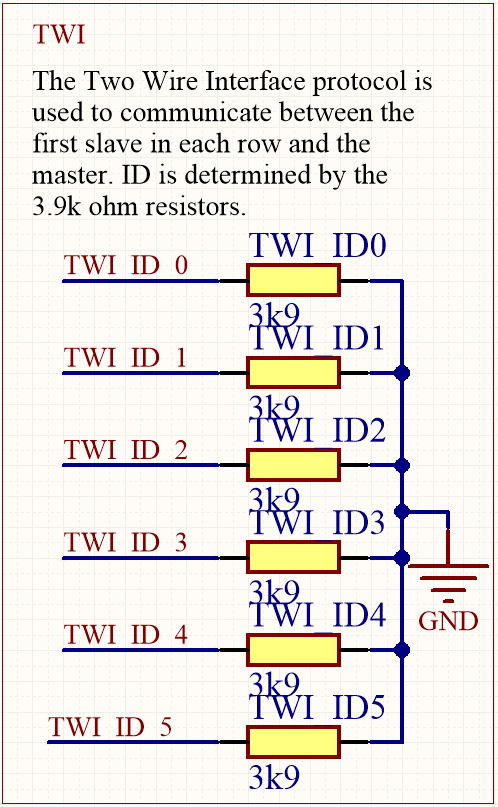
\includegraphics[width=0.3\textwidth]{05_My_Implementation/figures/TWI.png}
    \caption{Schematic over the setting of the TWI ID}
    \label{fig:my_label}
\end{figure}

There is a choise to use the daisy chained SPI to retrieve the ID's from one row at the time, leaving more time for the ATmega4809 to do other tasks.

\begin{figure}[H]
    \centering
    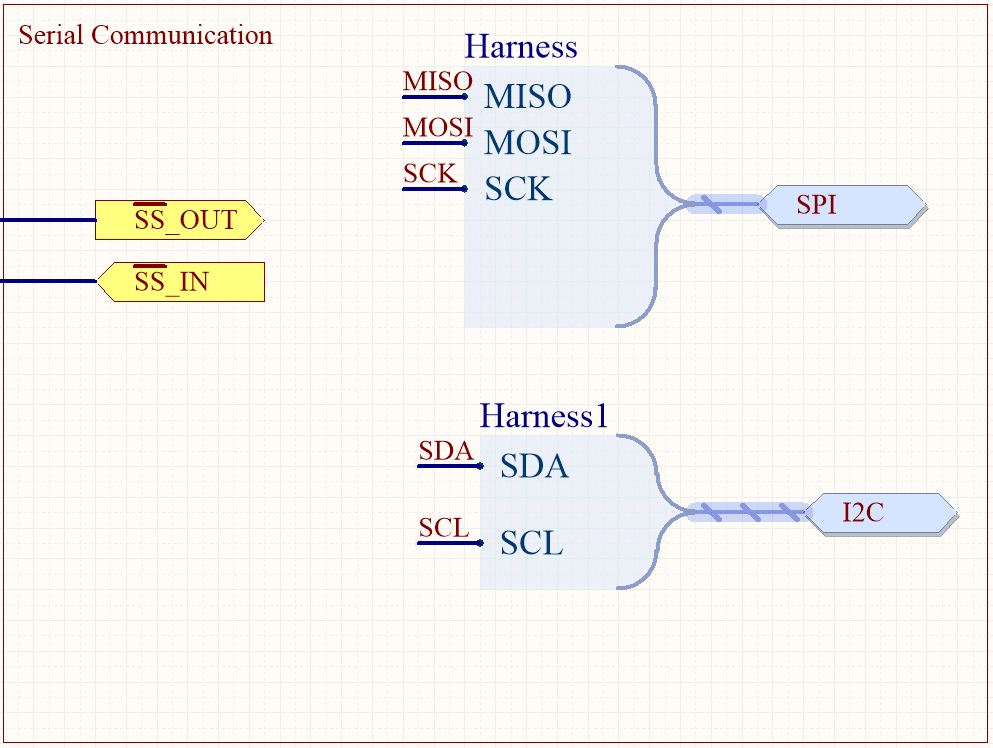
\includegraphics[width=\textwidth]{05_My_Implementation/figures/Serial.png}
    \caption{Serial communication between the ATtiny1617's and TWI to ATmega4809}
    \label{fig:my_label}
\end{figure}

\subsection{MCU}


As stated in Chapter \ref{proposedSolution} the AVR chosen for the RFID circuit is a ATtiny1617\cite{attiny1617}. The main reason for this is that it is one of the newest ATtiny's and the fact that it has three AC's, from which two are in use. Main features that is used are include:


\


\subsection{Pins used}
For debug purposes, all the pins are populated. In this design, the only pins which are required to operate the RFID are 
\begin{table}[H]
\centering
\caption{Pins used for RFID}
\label{tab:RFID_pins}
\begin{tabular}{lll}
\hline
PIN & Name   & Function                   \\
\hline
PA7 & AC\_IN & Input for the RFID tag     \\
PB3 & 125KhZ & Wave form generator output \\
\hline
\end{tabular}
\end{table}

Port C of the MCU is used to physically set the TWI (Microchips I$^2$C equivalent) ID, so that you do not need to run different programs on each separate MCU.

Furthermore two different approaches are implemented to talk to the individual slaves. All slaves are equipped with TWI, so that you can talk to them individually. Alternatively one can choose to only enable TWI on the 8 end nodes, the one closest to the LDO (REF FIGURE HERE) and let this talk on SPI to the rest of the nodes on that PCB, subsequently reporting all RFID chips detected to the master.

\begin{figure}[H]
    \centering
    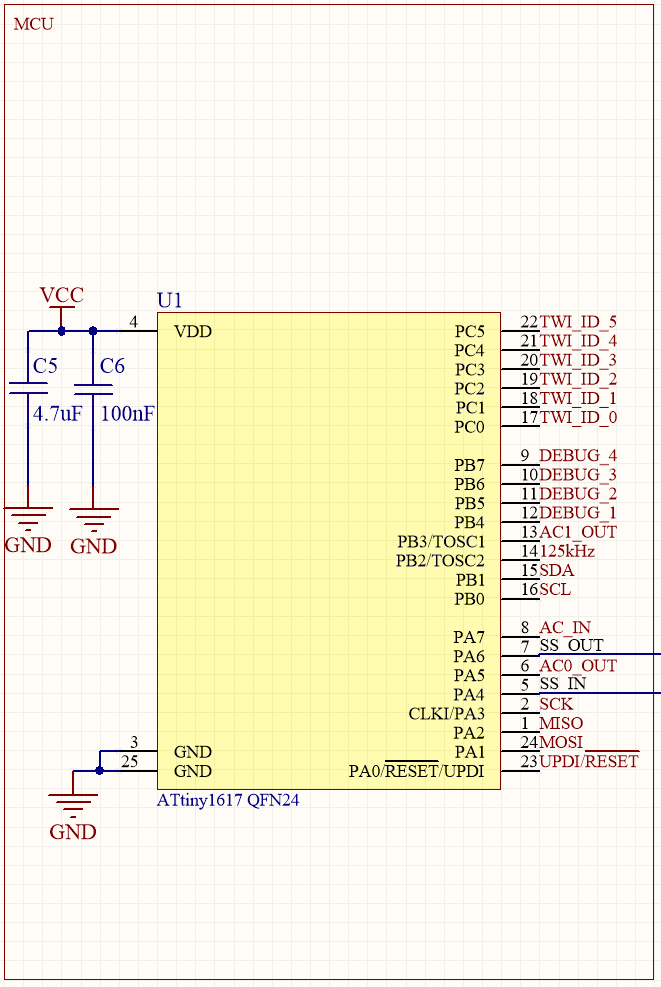
\includegraphics[width=\textwidth]{05_My_Implementation/figures/MCU.png}
    \caption{The MCU connections and net names.}
    \label{fig:05:MCU}
\end{figure}


\subsection{Debugging}
Having a lot of free pins, a good use of them can be to output interesting data. Pads are placed so that one can read out the AC output, AC input, 125 kHz generator wave and peak detector. If anything is wrong with a node, it should be possible to find out by probing these points in order to diagnose the problem.
\begin{figure}[H]
    \centering
    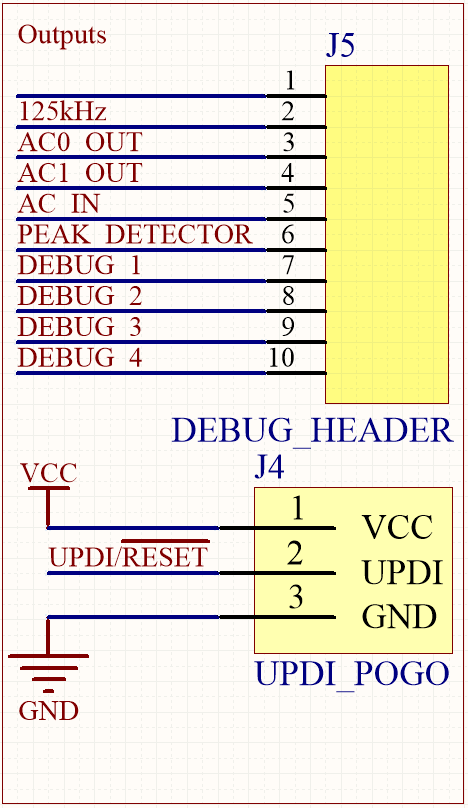
\includegraphics[width=0.3\textwidth]{05_My_Implementation/figures/Outputs.png}
    \caption{Schematic over the probing/programming pads}
    \label{fig:05:outputs}
\end{figure}


\begin{table}[H]
\centering
\caption{Overview of probing points for debugging}
\label{PinDebug}
\begin{tabular}{lll}
\hline
PIN & Name          & Function for debugging                                                    \\
\hline
PB2 & 125kHz        & Making sure the MCU is toggling the transistor correctly. \\
PA5 & AC0\_OUT      & See if we have any false triggering on the falling edge.  \\
PB3 & AC1\_OUT      & See if we have any false triggering from the rising edge.   \\
PA7 & AC\_IN        & See if the signal sent into the AC is clean, and plausible.               \\
-   & Peak-detector & See if there are some errors in the peak-detector                        \\
PB4 & Debug 1       & Future-proof in case more output is needed                                \\
PB5 & Debug 2       & Future-proof in case more output is needed                                \\
PB6 & Debug 3       & Future-proof in case more output is needed                                \\
PB7 & Debug 4       & Future-proof in case more output is needed                                \\
\hline
\end{tabular}
\end{table}

\newpage
\section{PCB design}
\todo{Fill section}

\begin{figure}[H]
    \centering
    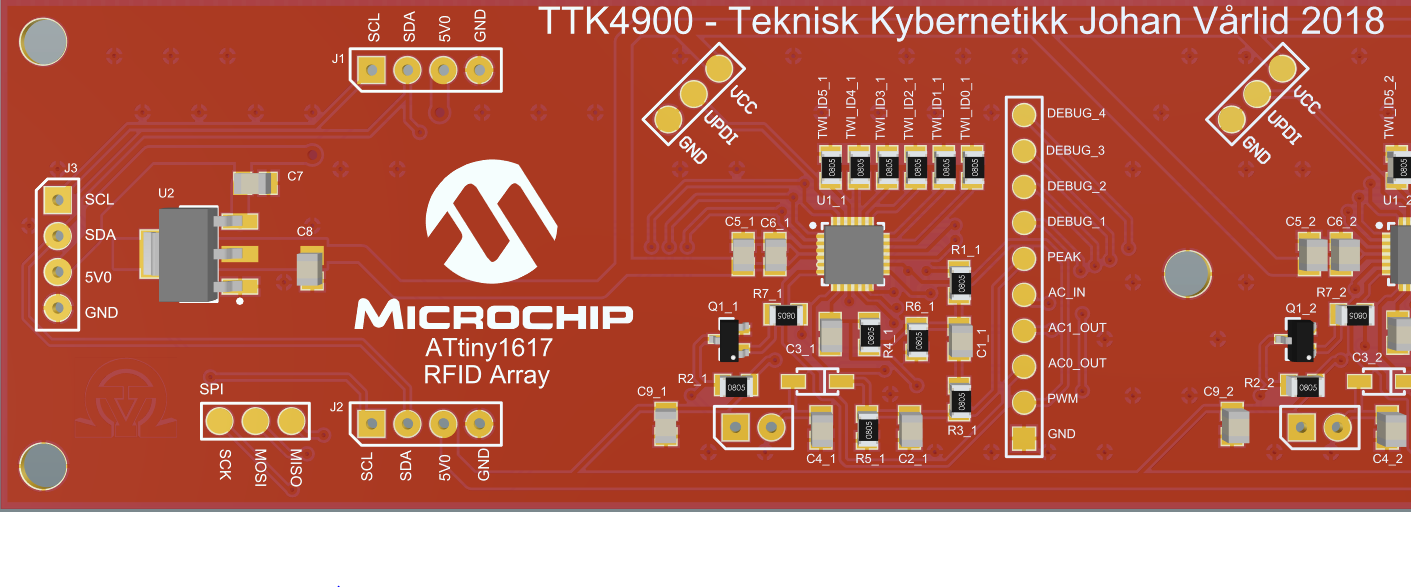
\includegraphics[width=\textwidth]{05_My_Implementation/figures/PCB-3D-Render.png}
    \caption{3D rendering of power supply for each plank and one reader}
    \label{fig:3D_PCB_Small}
\end{figure}

\section{Power distribution}
\todo{Fill section}
\section{Chessboard}
\todo{Fill section}
\cite{roberti_francois}
\begin{table}[H]
\centering
\caption{Minimum height of the chamber inside the chessboard}
\label{my-label}
\begin{tabular}{lll}
\hline
Part                    & Height & Placement    \\
\hline
Antenna                 & 2mm    & Under spacer \\
LED wires               & 2mm    & Under spacer \\
Spacers                 & 12mm   & -            \\
PCB                     & 1.6mm  & Over spacer  \\
Tallest component       & 6.6mm  & Over spacer  \\ 
Total minimum height    & 20.2mm & -            \\ 
\hline
\end{tabular}
\end{table}

\section{ATmega4809}
\cite{atmega4809}

\section{WINC1500}

A resent co-operation with Google made use of the ATmega 4809 and the WINC1500 to make it easy to connect an embedded system to Google's cloud systems 


\section{MQTT}

As a MQTT message broaker, the service that coordinates all the traffic between the devices much like a server, \textit{Eclipse Mosquitto} is used. \cite{mosquitto} This was downloaded to my server at NTNU, \url{inkognito.ed.ntnu.no} and can be reached on port 1833. Here, the FEN of a chessboard can be published to the topic "chess".\\

Snapping up the messages sent form the board, a simple python script rewritten from a Python Software Foundation example. \cite{mqttpython} This can be found as \texttt{Programs/mqtt\_client.py} in the zip. It simply takes whatever it gets, and overwrites the file \texttt{state}.\\

\section{Chessboard online feed}

To be able to see the current state of the chessboard, a web service based on Niklas Fiekas GitHub repository web-boardimage is used. \cite{Fiekas2017} It checks the file \texttt{state} for a change every 2 ms. After a change occures, it takes about 200ms to generate a new picture and load the page for the user. The loading, of course, depends on the users connection. The actual generation times seems to rely on the amount of pieces on the board, as it has to generate a small picture to represent each piece on each tile. The code for this site can be found under \texttt{www/web-boardimage}.